\setchapterimage[2cm]{../images/header-sunflowers.jpg}
%\setchapterpreamble[u]{\margintoc}
\chapter{The sunflower molecules}
\labch{sunflowers}


\section{Introduction and origin}

The search for effective and interesting SERS substrates ended up leading us to a novel class of molecules researched and presented in the year 2006 by Chernichenko and his colleagues.\sidecite{chernichenko06}
The first representative of this family, nicknamed as \q{sulflower}, is the ocatathio[8]circulene.
This highly symmetric structure, which may be described as a form of carbon sulfide and as a belt of annulated thiophene cycles, is claimed to have great stability, high symmetry and unusual electronic properties.

\begin{marginfigure}
    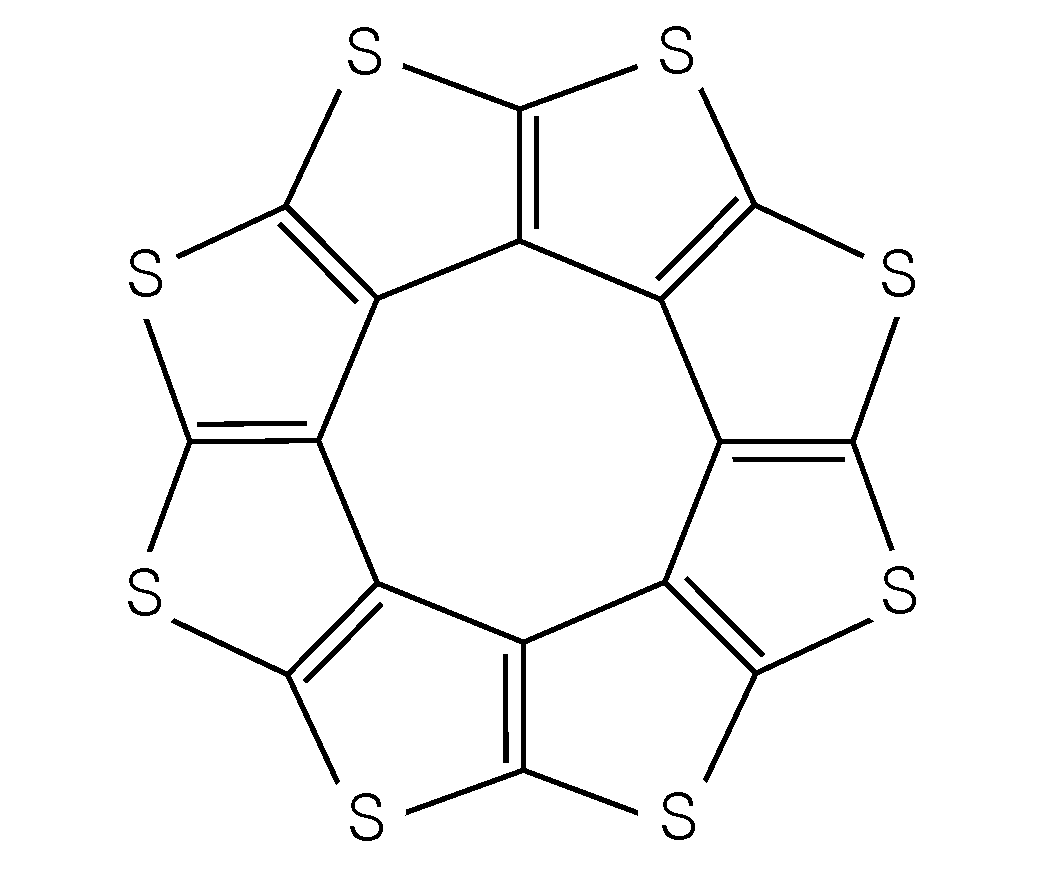
\includegraphics{sulflower-structure}
    \caption[Structure of sulflower]{Structure of sulflower}
    \labfig{sulflower-structure}
\end{marginfigure}


From a synthetic point of view, sulflower also proved to be simple and straightforward to develop despite its complex appearance: starting from tetrathiophene, sulphurizing its free sites and acidificating ot get polythiol, and removing the excess sulfur by vacuum pyrolysis.
This process allowed the team to achieve yields of 56\% starting from commercially available reagents.

Interestingly, the team proposes that it could be possible to prepare materials with diverse electronic properties by using different types of heteroatoms and varying on the basic structure of the molecule.
Such a statement made apparent the potential of this family of molecules: highly symmetrical, stable, surface-like structures with variable electronic behavior could act as suitable SERS substrates.
This chapter is entirely dedicated to that premise: the study and characterization of sulflower and sulflower-like molecules, which from now on I will collectively refer to as \q{sunflowers}.
By designing, generating and studying our own family of sunflowers, we will be contributing to characterize a novel and interesting group of molecules, and we may be able to identify an ideal SERS environment for STX.


\section{Sunflower design}

\begin{marginfigure}
    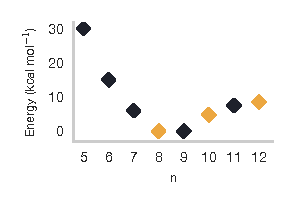
\includegraphics{sulflower-strain}
    \caption[Strain of thiophenic circulenes]{Strain of thiophenic circulenes with n rings}
    \labfig{sulflower-strain}
\end{marginfigure}

To start designing a family of molecules, first we must clearly state their defining pattern.
For this purpose, we adopt Chernichenko et al.'s own proposal: \q{a novel class of heterolytic circulenes}.
We start expanding the model by answering the question: are thiophene based circulenes with other than 8 rings stable enough to be worth considering?
The answer is in the original paper itself.
\reffig{sulflower-strain}, which was recreated to use our calculation level and adapt to the style of the document, shows that 8 ring structures are the most stable alongside 9.
The details about this calculation are further explained in \refsec{study-of-stability}.
However, considering their low relative energies and the fact that they have an even number of electrons (which would greatly simplify later calculations), 10 and 12 ring sunflowers were also chosen as part of the study.

Expanding upon this idea to allow for further heteroatom substitution, we ended up with the templates in \reffig{sunflower-skeletons}.
The possibilities were numerous, but we settled for S, Se, As and P substitutions on X$_1$ sites, and N substitutions in some cases in X$_2$ sites.
A full table detailing all of the structures that were generated and will comprise this study can be found in \reftab{sunflower-family}, as well as the short names or IDs that were given to each species based on its composition and number of petals for the sake of abbreviation.

\begin{figure*}
    \centering
    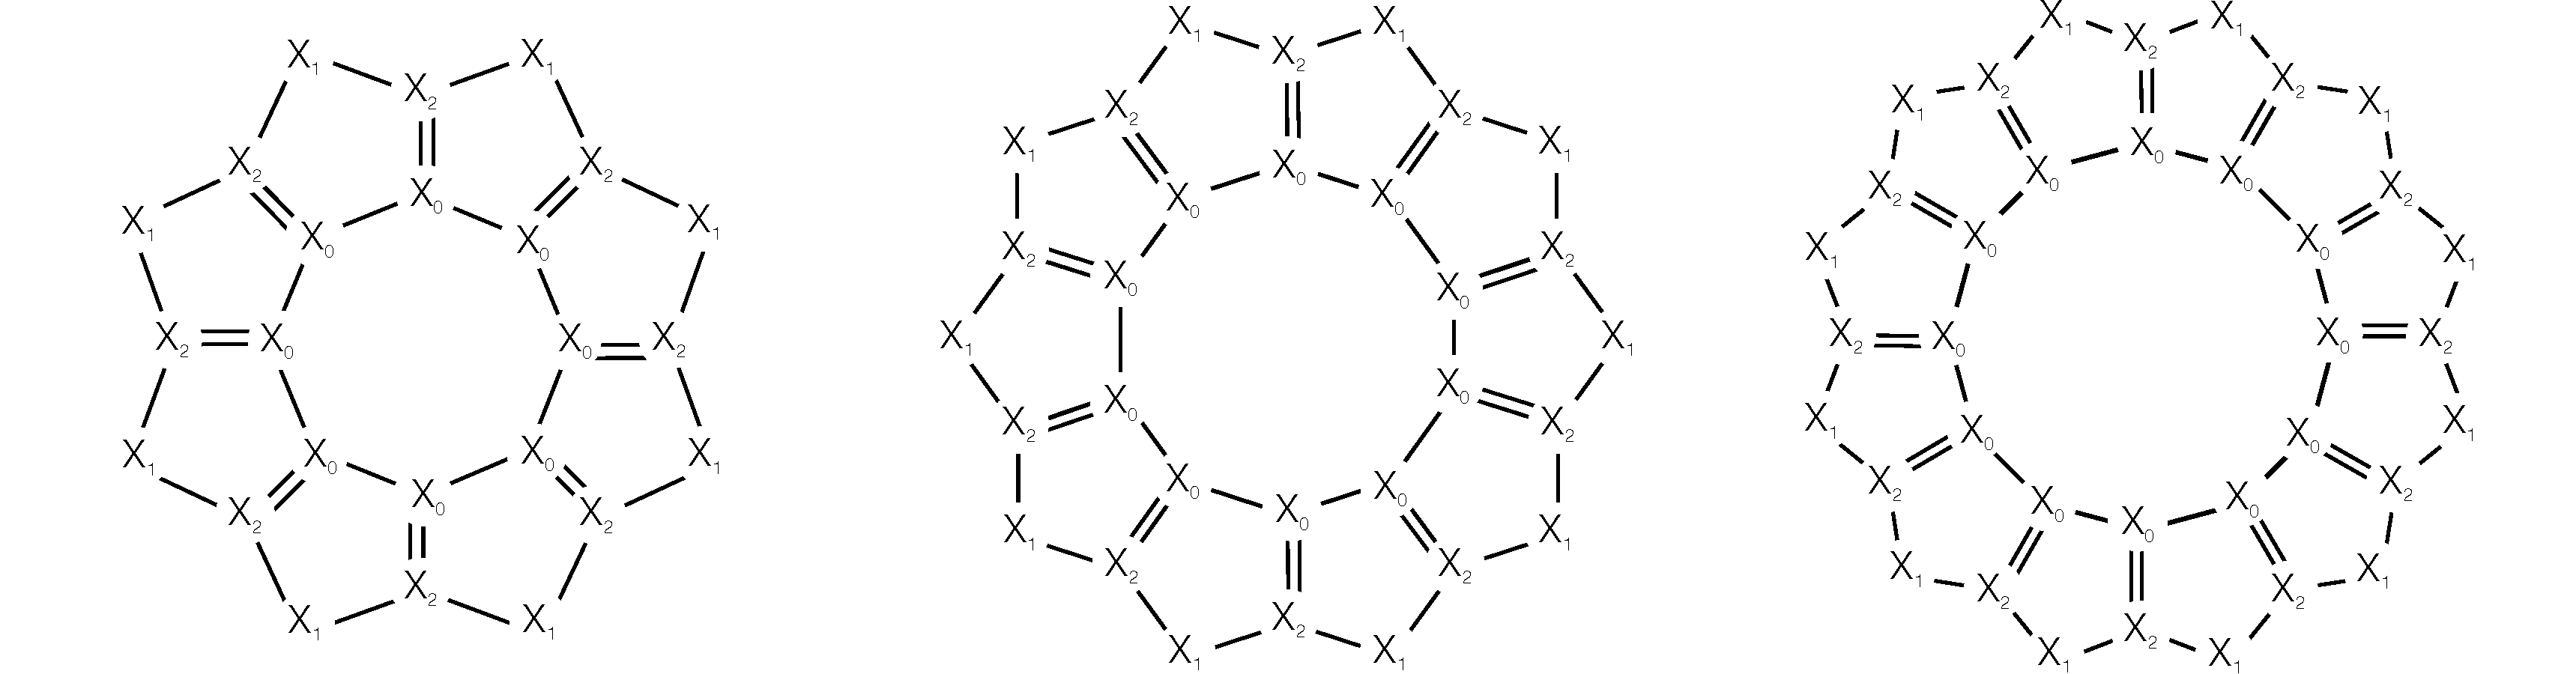
\includegraphics{sunflower-skeletons}
    \caption[General structures of the sunflower family]{From left to right, general structures of the 8, 10 and 12 ring sunflowers}
    \labfig{sunflower-skeletons}
\end{figure*}

\begin{table}
    \centering
    \caption[Sunflowers in this study]{Subset of the sunflower family that is going to be studied}
    \begin{tabular}{@{}cccrrr@{}}
        \toprule
        &&& \multicolumn{3}{c}{number of rings} \\
        X$_0$ & X$_1$ & X$_2$ & \multicolumn{1}{c}{8} & \multicolumn{1}{c}{10} & \multicolumn{1}{c}{12} \\
        \midrule
        C & S & C & S08 & S10 & S12 \\
        C & Se & C & Se08 & Se10 & Se12 \\
        C & As & C & As08 & As10 & As12 \\
        C & As & N & AsN08 & AsN10 & AsN12 \\
        C & P & C & P08 & P10 & P12 \\
        C & P & N & PN08 & PN10 & PN12 \\
        \bottomrule
    \end{tabular}
    \labtab{sunflower-family}
\end{table}


\section{Study of geometry}
\labsec{study-of-geometry}

\begin{marginfigure}
    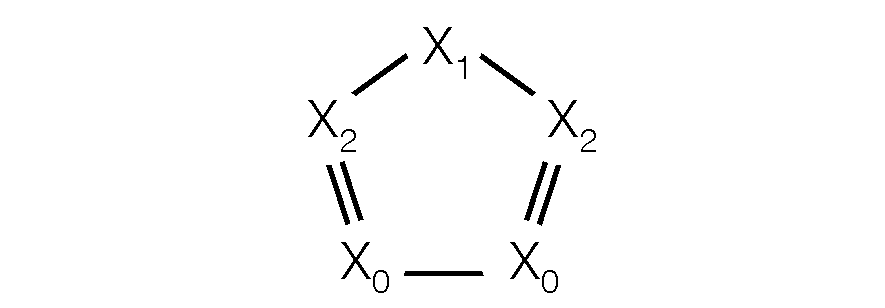
\includegraphics{pentagon-structure}
    \caption[Thiophene-like structure template]{Thiophene-like structure template (hydrogen is added to adjust for neutrality as needed)}
    \labfig{pentagon-structure}
\end{marginfigure}

Coordinate files for all of the designed sunflowers were created using 3D molecule modeling software.
Then, they were optimized at the M06-2X/def2SVP calculation level.

\begin{figure}
    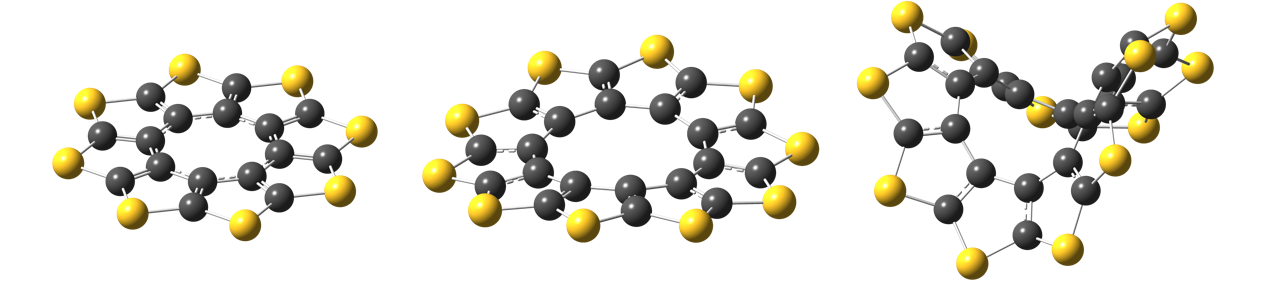
\includegraphics{sunflower-shapes}
    \caption[Shape of the sunflowers]{Shape of optimized S08, S10 and S12, from left to right (note the progressive increase in their deviation from planarity)}
    \labfig{sunflower-shapes}
\end{figure}

Using the output files for these calculations, all of the bond distances in all of the systems were extracted using Python.
Then, the bonds were grouped by type: inner (I, bonds between X$_0$ atoms, which were carbon in all cases), middle (M, between X$_0$ and X$_2$ atoms, which were either C-C or C-N bonds), and outer (O, between X$_2$ and X$_1$ atoms).
The mean and standard deviation (SD) of these groups was computed for all of the flowers.
Additionally, thiophene-like pentagonal structures of the form displayed in \reffig{pentagon-structure} were modeled and optimized, and their bond length data was compared with the rest and presented in \reftab{bond-length-study}.

How is this information useful?
In the first place, it allows us to easily compare the average length of each bond type as the number of units increases.
More interestingly, it serves as a way to assess the nature of each bond group.
Take the inner C-C bonds.
In all cases, the average length lies between the usual values for single and double C-C bonds,\marginnote{\SI{1.54}{\angstrom} for single and \SI{1.34}{\angstrom} for double bonds \fix{add reference}} an information that immediately suggests us that the flowers might be conjugated systems with $\pi$ electron delocalization.
However, it could also be possible that there were equal amounts of single and double bonds, and that these apparently conjugated bond lengths were just a the result of a lousy statistical approximation.
That's why the SD metric was also computed.
Groups with a relatively high SD such as the I bonds of As08, As12, P08 and P12 are actually composed of longer and shorter bonds, and it's likely that their $\pi$ electrons aren't delocalized.
On the other hand, groups with small SD values are more likely to correspond to conjugated systems, which may be stabilized by electron delocalization.
This concept of bond length equalization and conjugation may be tied to that of aromaticity, where equalized C-C bonds could be a sign of it, and uneven ones could indicate non aromaticity or antiaromaticity.\sidecite{zhongfang05} This topic will be covered in greater detail in \refsec{study-of-aromaticity}.

\begin{table}
    \centering
    \caption[Bond length study]{Bond length statistics for each studied species, units are \si{\angstrom}}
    \begin{tabular}{@{}rlcccccc@{}}
        \toprule
        && \multicolumn{2}{c}{I (X$_0$-X$_0$)} & \multicolumn{2}{c}{M (X$_0$-X$_2$)} & \multicolumn{2}{c}{O (X$_1$-X$_2$)} \\
        && mean & std & mean & std & mean & std \\
        \midrule
        \multirow{4}{*}{S} & ring & 1.429 & - & 1.367 & 0.000 & 1.719 & 0.000 \\
        & 08 & 1.423 & 0.000 & 1.377 & 0.000 & 1.754 & 0.000 \\
        & 10 & 1.482 & 0.000 & 1.399 & 0.000 & 1.712 & 0.000 \\
        & 12 & 1.466 & 0.004 & 1.389 & 0.000 & 1.732 & 0.004 \\
        \\
        \multirow{4}{*}{Se} & ring & 1.434 & - & 1.363 & 0.000 & 1.857 & 0.000 \\
        & 08 & 1.454 & 0.000 & 1.385 & 0.000 & 1.865 & 0.000 \\
        & 10 & 1.478 & 0.003 & 1.389 & 0.000 & 1.861 & 0.004 \\
        & 12 & 1.466 & 0.007 & 1.381 & 0.000 & 1.877 & 0.005 \\
        \\
        \multirow{4}{*}{As} & ring & 1.468 & - & 1.354 & 0.000 & 1.918 & 0.000 \\
        & 08 & 1.434 & 0.050 & 1.448 & 0.000 & 1.859 & 0.008 \\
        & 10 & 1.436 & 0.000 & 1.454 & 0.001 & 1.856 & 0.001 \\
        & 12 & 1.435 & 0.042 & 1.446 & 0.002 & 1.867 & 0.007 \\
        \\
        \multirow{4}{*}{AsN} & ring & 1.495 & - & 1.283 & 0.000 & 1.854 & 0.000 \\
        & 08 & 1.434 & 0.000 & 1.361 & 0.000 & 1.858 & 0.000 \\
        & 10 & 1.450 & 0.001 & 1.364 & 0.001 & 1.856 & 0.004 \\
        & 12 & 1.440 & 0.004 & 1.357 & 0.001 & 1.873 & 0.006 \\
        \\
        \multirow{4}{*}{P} & ring & 1.467 & - & 1.359 & 0.000 & 1.794 & 0.001 \\
        & 08 & 1.410 & 0.048 & 1.445 & 0.000 & 1.764 & 0.006 \\
        & 10 & 1.431 & 0.000 & 1.471 & 0.000 & 1.736 & 0.000 \\
        & 12 & 1.429 & 0.045 & 1.462 & 0.002 & 1.747 & 0.005 \\
        \\
        \multirow{4}{*}{PN} & ring & 1.485 & - & 1.293 & 0.000 & 1.707 & 0.000 \\
        & 08 & 1.404 & 0.000 & 1.364 & 0.000 & 1.752 & 0.000 \\
        & 10 & 1.448 & 0.000 & 1.385 & 0.000 & 1.715 & 0.001 \\
        & 12 & 1.435 & 0.002 & 1.378 & 0.001 & 1.732 & 0.004 \\
        \bottomrule
    \end{tabular}
    \labtab{bond-length-study}
\end{table}


\section{Study of stability}
\labsec{study-of-stability}

Using the output files from the previous step, specifically those from the initial optimization, calculations related to the energies of the flowers were performed in order to assess their stabilities.

\subsection{Ring strain}
\labsec{ring-strain}
Ring strain may be defined as a kind of instability that arises when angles of the bonds in a cyclic molecule deviate from their optimal values, which they would be able to adopt if they weren't coiled in the shape of a ring.
The energy associated to this phenomenon can serve as a way to compare the stabilities of flowers with different numbers of petals, as it was done in the original paper and reproduced in \reffig{sulflower-strain}.
Its calculation relies on the design of an homodesmotic reaction.
What does this mean?
In a homodesmotic reaction, the number of atoms and the type of hybridations in the products are the same as in the reactants.
Our goal is to devise a chemical equation where the strained structure appears in only one of its sides and the rest of the chosen molecules don't present any stray effects.\sidecite{vidalvidal18}
If we manage to create such an equation, the reaction energy will correspond to the strain, as the rest of the components of the energy should nullify themselves between the two sides of the reaction.

In this case, apart from the sunflower structure B, the equations that were designed included molecules A and C, non-cyclic structures composed of 3 and 2 petals. \marginnote{
	\begin{equation}
        \labeq{homodesmotic-equation}
        E_\text{strain} = \frac{E_B + nE_C - nE_A}{n}
	\end{equation}
} By following this reaction, which is fully displayed in \reffig{homodesmotic}, the strain energy was calculated as shown in \refeq{homodesmotic-equation}.

\begin{figure}
    \centering
    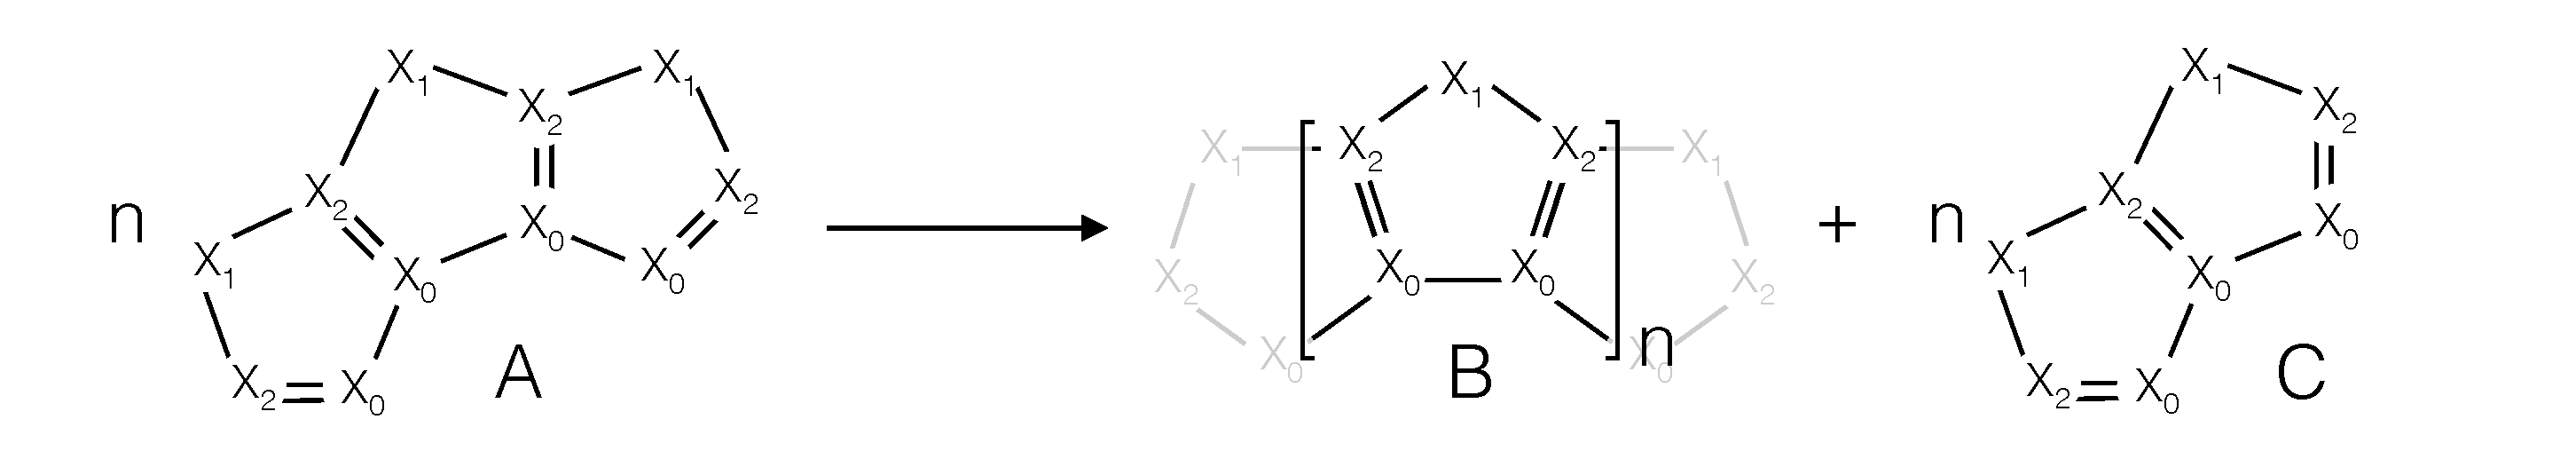
\includegraphics{homodesmotic}
    \caption[Homodesmotic reaction used to calculate strain energies]{Homodesmotic reaction used to calculate strain energies}
    \labfig{homodesmotic}
\end{figure}

This calculation, which is the one that was used to generate the previous sulflower stability curve \reffig{sulflower-stability}, was applied to all of the sunflowers of the study, and the resulting strain energies are presented in \reffig{sunflower-stability}.
As it can be seen, the strain energies always increase with the number of petals (as it's the case for the original sulflower series).
However, it may be noted that they increase following slightly different tendencies.
Notable examples are the P family, where the 8 and 10 petal species have very similar strains; and the Se, As and AsN families, where the energies of the 10 and 12 petal structures are very close.
These energy values are an useful indication of the relative strains of the different species within a family, and an estimation of their
stabilities with respect to the original sulflower.
Nevertheless, it should be kept in mind that this calculation is an approximation, and that the values of the so called strain energy might be accounting for other effects such as conjugation stabilization or \fix{maybe list another effect}.

\begin{figure}
    \centering
    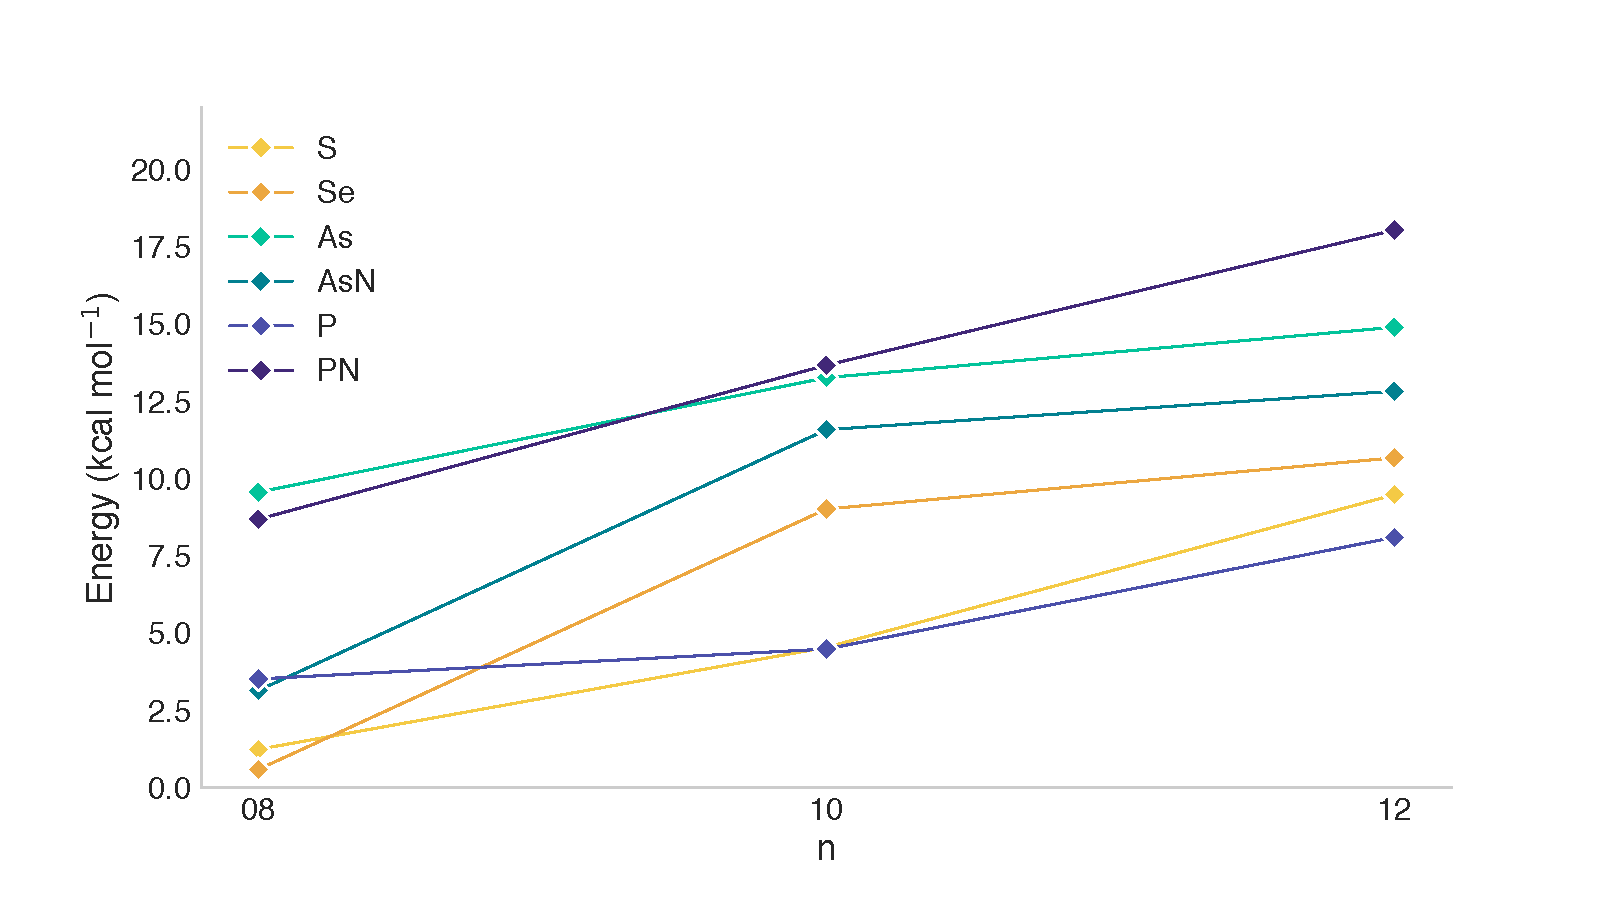
\includegraphics{sunflower-stability}
    \caption[Strain energies of sunflower groups]{Strain energies of all of the studied sunflower groups}
    \labfig{sunflower-stability}
\end{figure}

\blindtext


\section{Study of aromaticity}
\labsec{study-of-aromaticity}

Aromaticity is a property related to molecules that contain a ring or a chain of resonance bonds that increases their stability.
It’s typically found in flat ring structures, although the definition has been discussed and expanded since its initial association to benzene,\sidecite{faraday1825} and there are other varieties such as annulenic, azulenic, inorganic, homoaromatic, three-dimensional, $sigma$-electron, and even metallic electron aromaticity.\sidecite{zhongfang05}
Considering their ringed structure and possibly high conjugation, we wondered if the sunflowers could present any kind of aromatic tendencies.
Having already studied their degree of bond length equalization in \refsec{study-of-geometry}, we set out to assess their aromaticity from the point of view of their magnetic properties.

\subsection{Nucleus-Independent Chemical Shift (NICS)}
Since its introduction in 1996 by Schleyer et al.\sidecite{schleyer96}, NICS has become the most popular and widely used technique to estimate aromaticity in a quantitative way.
It's based on the study of electronic ring currents.
As the electrons in the possibly-aromatic systems have a certain degree of free circulation, an external magnetic field perpendicular to the main plane of the system is able to induce a ring current.
Said ring currents generate their own magnetic field, which can weaken or strengthen the effect of the external field, resulting in decreased or increased NMR chemical shifts.
Aromatic systems will experience shielding on the inside of the ring and deshielding on the outside.
Antiaromatic systems will experience the opposite.

\subsubsection{The basic application of NICS}
NICS is usually applied to single rings, and quantified by computing the absolute magnetic shielding at key locations.
This key location is usually one of the following: the center of the ring (calculated as the non-weighted mean of the positions of the heavy atoms), several points along a central axis perpendicular to the plane of the ring (calculated trivially in planar rings as the plane that passes through any three ring atoms), at several points on a grid perpendicular to the plane of the ring, or as three dimensional isosurfaces using dense grids.

\subsubsection{A custom solution for non-planar molecules}

\begin{marginfigure}
    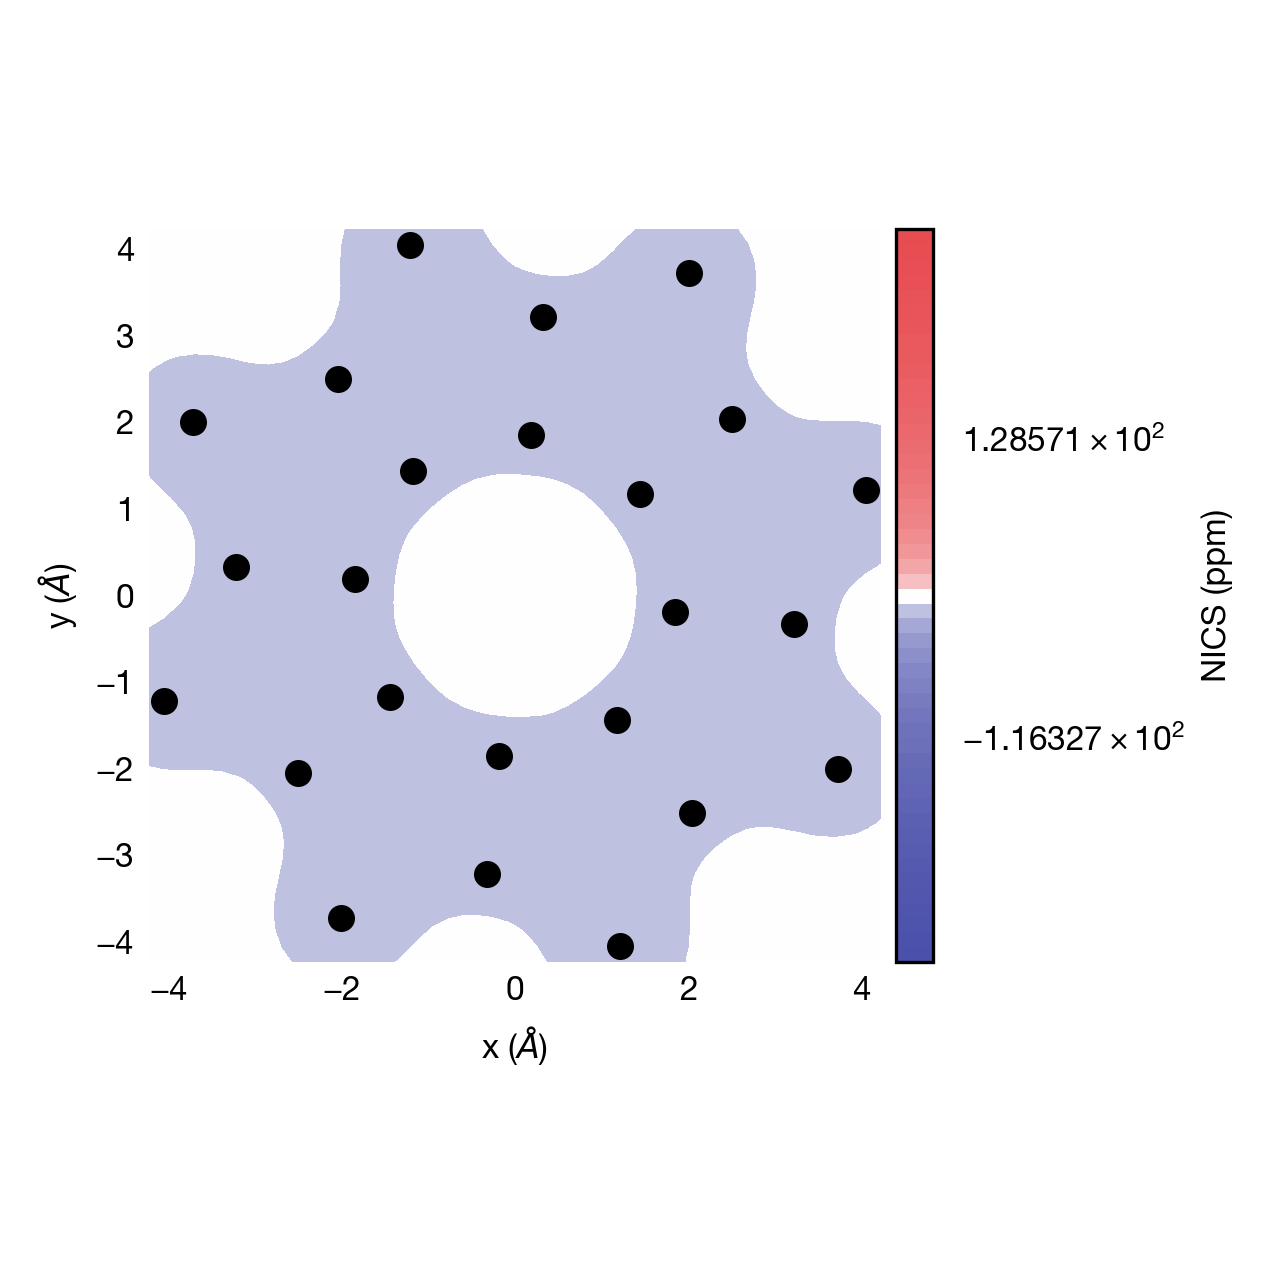
\includegraphics{nics-sample}
    \caption[NICS applied to sulflower]{Custom NICS technique applied to the original 8 petal sulflower molecule as a sample of the legacy approach}
    \labfig{nics-sample}
\end{marginfigure}

A seen in \reffig{sunflower-shapes} in \refsec{study-of-geometry}, 8 petal sunflowers are perfectly planar.
In previous studies, NICS calculations on flat grids parallel to their planes were applied with success.
The positive values of the magnetic shielding were plotted in red, and the negative ones in blue, which overlaid over the atoms of the flower, resulted in graphs like \reffig{nics-sample}.
However, 10 and 12 petal sunflowers have bended and warped shapes, and the \q{general plane} of the molecule is no longer a plane.
In order to translate the old method, a new approach was developed and applied.
The idea of extending a grid of points over the \q{general surface} of the molecule and plotting it as a 2D projection was maintained, but what was exactly a \q{general surface}, and how could it be generalized for non planar molecules?

\blindtext[8]

\subsection{AICD}
\subsubsection{The basics of AICD}
\blindtext
\subsubsection{Application and comparison of results}
\blindtext


\section{Spectroscopic characterization}

\subsection{Vibrational spectroscopy}
\subsubsection{Raman spectra}
\blindtext
\subsubsection{Decomposition of key modes}
\blindtext
\subsubsection{VEDA}
\blindtext

\subsection{Electronic spectroscopy}
\subsubsection{UV spectra}
\blindtext
